

Falls es sich hierbei um einen minimalen Schnitt handelt, dann würde dies bedeuten, dass eine ganzzahlige Lösung für $\overline{\mathcal{N}_G}$ existiert, mit deren Hilfe wir, zusammen mit $\varphi_z$, eine ganzzahlige zulässige Lösung für $\mathcal{N}_G$ konstruieren könnten, was wiederum ein Widerspruch zu unserer Annahme wäre. Es muss also einen kleineren Schnitt $\mathcal{S}_{min}$, mit $|\mathcal{S}_{min}| < |\overline{\mathcal{S}_1}|$, geben. 

\begin{claim} \label{cut_types1}

Ein minimaler Schnitt $\mathcal{S}_{min}$ in $\overline{\mathcal{N}_G}$ enthält ohne Beschränkung der Allgemeinheit nur Kanten von einem der vier Typen $\overline{E_\triangledown}, F_\square, V_*$ und $E_*$.

\end{claim}

Kanten auf einem Pfad von der Quelle bis zu einer Kante in $\overline{E_\triangledown}$, können durch diese ersetzt werden. Ebenso können Kanten zwischen zwei Winkeldreiecken, oder von einem Winkeldreieck zu einem kleinen Quadrat, durch die, entgegen dem Uhrzeigersinn, nächste Kante in $\overline{E_\triangledown}$ ersetzt werden. Kanten zwischen einem Kanten-Knoten und einem Knoten-Knoten, oder einem kleinen Quadrat, können durch eine Kante in $E_*$ ersetzt werden. Abschliessend können Kanten, von einem inneren Gebiet zu Senke, durch das hinzufügen von allen Kanten aus $F_\square$ an diesem Gebiet, ersetzt werden.

\begin{figure}[h]
	\centering
  	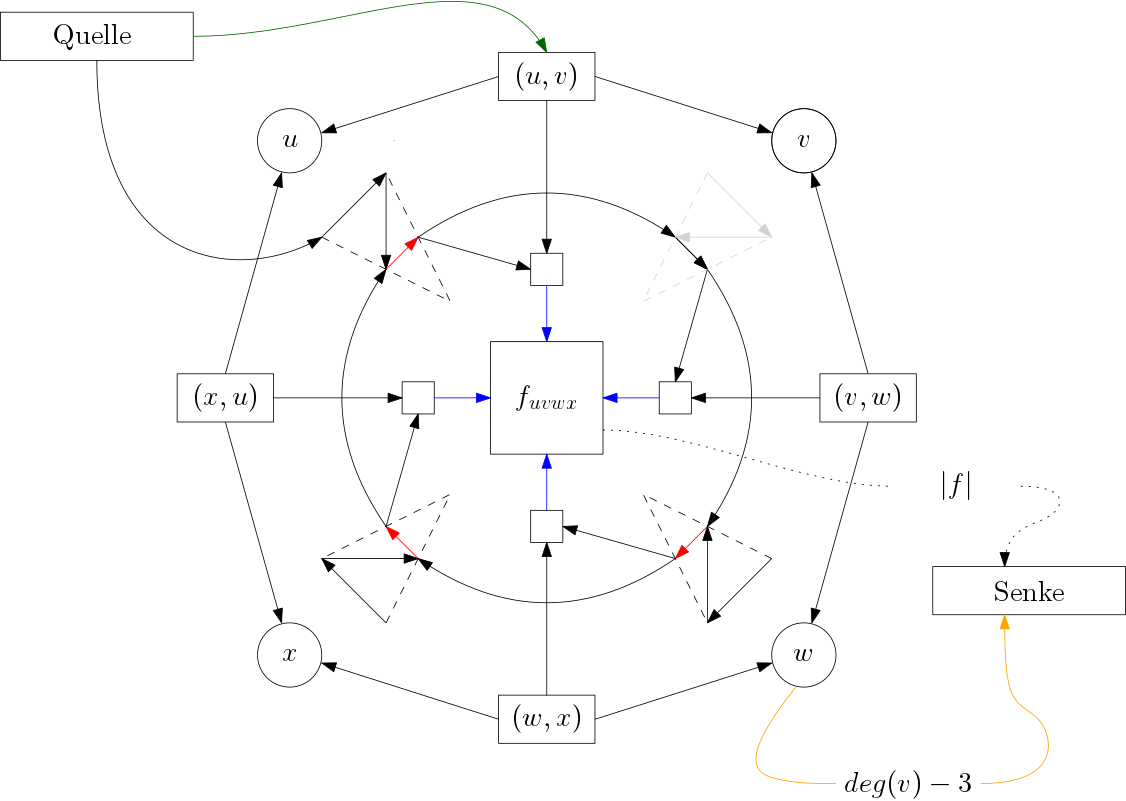
\includegraphics[width=0.7\textwidth]{face_cut.png}
  	\caption{Die vier Kantentypen $\overline{E_\triangledown}$ (rot), $F_\square$ (blau), $V_*$ (orange) und $E_*$ (grün) aus denen sich, nach Behauptungen \ref{cut_types1} und \ref{cut_types2}, ein minimaler Schnitt in $\overline{\mathcal{N}_G}$ zusammensetzt.}
\end{figure}

\begin{claim}\label{cut_types2}

Ein minimaler Schnitt $\mathcal{S}_{min}$ in $\overline{\mathcal{N}_G}$ muss ohne Beschränkung der Allgemeinheit aus jeder der Mengen $\overline{E_\triangledown}, F_\square, V_*$ und $E_*$ mindestens eine, aber aus keiner der Mengen alle Kanten enthalten.

\end{claim}

Falls ein solcher ein Schnitt existiert, dann kann er nicht alle Kanten $\overline{E_\triangledown}$ enthalten, da sonst $\mathcal{S}_{min} \cup E_z$ ein Schnitt in $\mathcal{N}_G$ wäre. Falls er jedoch keine Kante aus $\overline{E_\triangledown}$ enthält, dann muss er alle Kanten aus $F_\square$ enthalten. Falls er alle Kanten aus $F_\square$ enthält, dann muss er o.B.d.A. auch alle Kanten aus $V_*$ enthalten, und ist somit zu groß. Angenommen er enthält keine Kante aus $F_\square$, dann muss er alle Kanten aus $\overline{E_\triangledown}$ und $E_*$ enthalten, was ebenfalls ein Widerspruch wäre. Mit analogen Argumenten folgt der Rest von Behauptung \ref{cut_types2}. \\

Nehmen wir also an, dass ein minimaler Schnitt $\overline{E_\triangledown}$, wie in Behauptungen \ref{cut_types1} und \ref{cut_types2}, existiert mit $|\mathcal{S}_{min}| \leq 3|F_{in}| + |E_{in}| - 1$. Betrachten wir für den Moment das Teilnetzwerk um ein inneres Gebiet in $\overline{\mathcal{N}_G}$. Falls alle drei Kanten aus $\overline{E_\triangledown}$ in $\mathcal{S}_{min}$ enthalten sind, dann müssen auch o.B.d.A alle Kanten in $E_*$ um dieses Gebiet enthalten sein und falls eine Kante aus $\overline{E_\triangledown}$ nicht enthalten ist, dann müssen, im Uhrzeigersinn bis zur nächsten enthaltenen Kante aus $\overline{E_\triangledown}$, alle Kanten aus $F_\square$ Teil von $\mathcal{S}_{min}$ sein. Falls höchstens eine Kante aus $\overline{E_\triangledown}$ im Schnitt läge, dann folgt o.B.d.A, dass keine Kante aus $\overline{E_\triangledown}$ und alle aus $F_\square$ um das innere Gebiet enthalten sind. 

Angenommen es existieren nur Gebiete in denen entweder alle oder keine Kanten aus $\overline{E_\triangledown}$ in $\mathcal{S}_{min}$ enthalten sind. Dann existiert ein Kanten-Knoten der eines von beiden berührt.

\begin{figure}[h]
	\centering
  	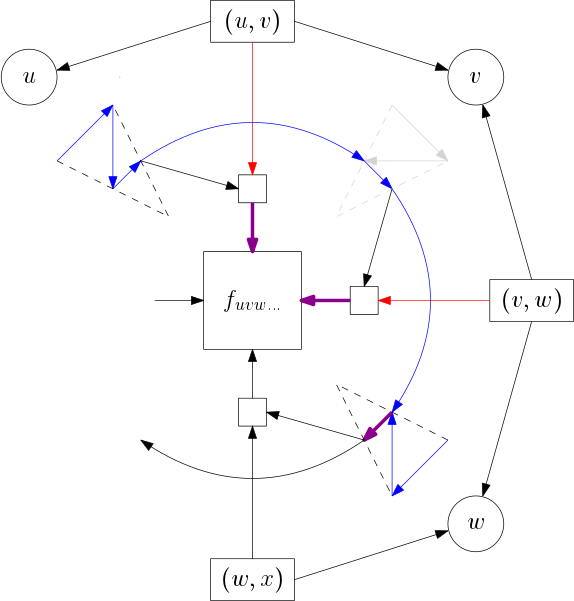
\includegraphics[width=0.7\textwidth]{face_cut_example.png}
  	\caption{}
\end{figure}



\begin{proof}
Da $\tilde{\varphi}$ ein zulässiger Fluss ist, muss $|\tilde{\varphi}_z| = \sum_{f \in F_{in}}(|f|-3)$ gelten. Seien $P_z$ die (nicht ganzzahligen) Pfade die zusammen $\tilde{\varphi}_z$ ergeben, dann gilt $|\tilde{\varphi}_z(p)| \in (0,1]$ für $p \in P_z$, wobei $|\tilde{\varphi}_z(p)|$ die Menge des Zuweisungsflusses entlang $p$ beschreibt. Es gilt $|P_z| \geq \sum_{f \in F_{in}}(|f|-3)$ und ebenso $|W| \geq \sum_{f \in F_{in}}(|f|-3)$.

Sei $\phi$ die Menge der zugewiesenen Winkel $(f_{aus},v)$ im äusseren Gebiet. Betrachte ein inneres Gebiet $f$. Dann führen mindestens $|f|-3$ Pfade $p \in P$ durch $f$. Wähle nun $|f|-3$ dieser Pfade $\{p_1, \dotsc , p_{|f|-3}\} = P_f$ aus und füge die zugehörigen Winkel $\{(f,v_1), \dotsc , (f,v_{|f|-3})\} = W_f \subseteq W$, zu $\phi$ hinzu. Lösche nun alle Winkel $(f',v)\in \tilde{W}_f$ aus $W$ die Knoten $\{v_1, \dotsc , v_{|f|-3}\}$ enthalten und alle Pfade $\tilde{P}_f$ aus $P$ die durch ihre Dummy-Knoten $\{v^*_1, \dotsc , v^*_{|f|-3}\}$ laufen. Dann gilt $|\varphi_z(\tilde{P}_f)| \leq |f|-3$ und somit $|\varphi_z(P\backslash P_v)| \geq |\varphi_z(P)| - |f| + 3$. Für $W \backslash \tilde{W}_f$ folgt ebenfalls $|W \backslash \tilde{W}_f| \geq |\varphi_z(P)| - |f| + 3$, da an jedem anderen von $\varphi_z$ genutzten $v^*$ noch mindestens ein Winkel aus $W\backslash \tilde{W}_f$ liegt. 
Es bleibt zu zeigen, dass für jedes andere Gebiet $f'$ mindestens $|f'|-3$ Winkel in $W\backslash \tilde{W}_f$ übrig sind. zwei Innere gebiete haben nur eine gemeinsame Kante und somit nur zwei gemeinsame Dummy-Knoten $v^*_1,v^*_2$.  
Wir können diesen Schritt somit insgesamt $|F_{in}|$ mal durchführen und jeder Knoten ist nur in einem Winkel aus $\phi$ enthalten. Es folgt $|\phi| = \sum_{f \in F_{in}}(|f|-3) + |f_{aus}| - 3 = \sum_{f \in F}(|f|-3)$. Die so erhaltene Menge $\phi$ entspricht also einem FAA von $G$.
\end{proof}
